\documentclass[11pt, a4paper]{article}
\usepackage{mwe}
\usepackage{amsmath, amssymb}
\usepackage{mathtools}
\usepackage{graphicx}
\graphicspath{{"../figures/"}}
\usepackage[section]{placeins} % to keep figures in their sections
\usepackage[export]{adjustbox} % for subcaptionbox figures

\usepackage{xcolor}
\usepackage{bm} % for bold vectors in math mode
\usepackage{physics} % for differential notation, etc...
\usepackage[separate-uncertainty=true]{siunitx}

\usepackage[most, minted]{tcolorbox} % for displaying code

\newtcblisting{python}{%
	listing engine=minted,
	minted language=python,
	listing only,
	breakable,
	enhanced,
	minted options = {
		linenos, 
		breaklines=true, 
		tabsize=2,
		fontsize=\footnotesize, 
		numbersep=2mm
	},
	overlay={%
		\begin{tcbclipinterior}
			\fill[gray!25] (frame.south west) rectangle ([xshift=4mm]frame.north west);
		\end{tcbclipinterior}
	}   
}

\newtcblisting{matlab}{%
	listing engine=minted,
	minted language=matlab,
	listing only,
	breakable,
	enhanced,
	minted options = {
		linenos, 
		breaklines=true, 
		tabsize=2,
		fontsize=\footnotesize, 
		numbersep=2mm
	},
	overlay={%
		\begin{tcbclipinterior}
			\fill[gray!25] (frame.south west) rectangle ([xshift=4mm]frame.north west);
		\end{tcbclipinterior}
	}   
}

\usepackage[margin=3cm]{geometry}
\usepackage[colorlinks = true,
            linkcolor = blue,
            urlcolor  = blue,
            citecolor = blue,
            anchorcolor = blue]{hyperref}

\setlength{\parindent}{0pt} % to stop indenting new paragraphs
\newcommand{\diff}{\mathop{}\!\mathrm{d}} % differential
\newcommand{\eqtext}[1]{\qquad \text{#1} \qquad}
\newcommand{\mat}[1]{\mathbf{#1}}
\renewcommand{\vec}[1]{\bm{#1}}

\newcommand{\diag}{\operatorname{diag}}
\newcommand{\off}{\operatorname{Off}}
\newcommand{\schro}{Schr\"{o}dinger\xspace}

\begin{document}
\title{The Symmetric Eigenvalue Problem}
\author{Elijan Jakob Mastnak\\[1mm]\small{Student ID: 28181157}}
\date{October 2020}
\maketitle

\tableofcontents

\newpage
\begin{center}
\textbf{Assignment}
\end{center}
Diagonalize and find the eigenvalues, eigenvectors and eigenfunctions of the perturbed Hamiltonian $ H = \frac{p^{2}}{2} + \frac{q^{2}}{2} + \lambda q^{4}$ for $ \lambda \in [0, 1]$ (explained in the \hyperref[eigen:s:solution]{theory section}). Diagonalize the matrix $ \bra{i}H\ket{j} $ using multiple diagonalization algorithms---be sure to implement at least some of the algorithms ``by hand''. Confirm that $ E_{n} \to E_{n}^{0} $ in the limit $ \lambda \to 0 $. 

Investigate the dependence of $ H $'s eigenvalues and eigenfunctions on the matrix's dimension $ N $. Investigate the convergence of the eigenvalues for large $ N $. 

\vspace{2mm}
\textit{Optional:} Perform a similar analysis of the ``double-well'' Hamiltonian
\begin{equation*}
	H_{\text{DW}} = \frac{p^{2}}{2} - 2q^{2} + \frac{q^{4}}{10},
\end{equation*}
which describes a particle in a potential with a double minimum. 


\vspace{2mm}

\rule{\textwidth}{0.2pt}


\section{Theory} \label{eigen:s:theory}
\vspace{-2mm}
\textit{To jump right to the solution, see \hyperref[eigen:s:solution]{Section \ref{eigen:s:solution}}}.


\subsection{Unperturbed Hamiltonian}
In dimensionless form, with energy measured in units of $ \hbar \omega $, momentum in units of $ (\hbar \omega m)^{1/2} $, and length in units of $ \big(\frac{\hbar}{m \omega}\big)^{1/2} $, the one-dimensional quantum harmonic oscillator's Hamiltonian is
\begin{equation}
	H_{0} = \frac{1}{2}(p^{2} + q^{2}) \label{eigen:eq:H0}
\end{equation}
The unperturbed Hamiltonian eigenstates $ \ket{n^{0}} $ are
\begin{equation}
	\ket{n^{0}} = \big(2^{n}\sqrt{\pi}n!\big)^{-1/2}e^{-\frac{q^{2}}{2}}\mathcal{H}_{n}(q) \label{eigen:eq:qho-basis}
\end{equation}
where $ \mathcal{H}_{n} $ denotes the $ n $th Hermite polynomial. These eigenstates satisfy the stationary \schro equation
\begin{equation*}
	H_{0}\ket{n^{0}} = E_{n}^{0}\ket{n^{0}}, \quad  n = 0, 1, 2, \ldots
\end{equation*} 
where $ E_{n}^{0} = n + \frac{1}{2} $ are the Hamiltonian's non-degenerate eigenvalues in units of $ \hbar \omega $. The associated $ (N \cross N) $ matrix $ H_{0} $ with elements $ \bra{i}H_{0}\ket{j} $, where $ i,j = 0, 1, 2, \ldots, N-1 $, is diagonal, with matrix elements $ \delta_{ij}(i + \frac{1}{2}) $. 

\subsection{Perturbed Hamiltonian}
We add a perturbation term $ \lambda q^{4} $ to $ H_{0} $ (Equation \ref{eigen:eq:H0}) to get the perturbed Hamiltonian
\begin{equation*}
	H = H_{0} + \lambda q^{4} = \frac{1}{2}(p^{2} + q^{2}) + \lambda q^{4}
\end{equation*}
where the perturbation parameter $ \lambda $ varies from e.g. 0 to 1. We then ask how the perturbation term changes the original Hamiltonian's energy eigenvalues. Namely, we are interested in the perturbed Hamiltonian $ H $'s matrix elements $ \bra{i}H\ket{j} $ expanded in the basis of unperturbed eigenstates $ \ket{n^{0}} $. We end up solving the eigenvalue problem 
\begin{equation*}
	H\ket{n} = E_{n} \ket{n}
\end{equation*}
where the perturbed eigenfunctions $ \ket{n} $ are linear combinations of $ \ket{n^{0}} $.

\subsection{Perturbation Matrix Elements}
There are a few options for constructing the perturbation matrix $ Q^4 $:
\begin{enumerate}
	\item Find the expected value of $ q_{ij} = \bra{i}q\ket{j} $ and construct $ Q^4 \to [q_{ij}]^{4} $
	\item Find $ (q^{2})_{ij} = \bra{i}q^{2}\ket{j} $ and construct $ Q^{4} \to [(q^{2})_{ij}]^{2}  $
	\item Find $ (q^{4})_{ij} = \bra{i}q^{4}\ket{j} $ and construct $ Q^{4} \to [(q^{4})_{ij}] $
\end{enumerate} 
The expected values of the matrix elements are
\begin{align}
	&q_{ij} = \frac{1}{2} \sqrt{i + j + 1} \delta_{\abs{i-j}, 1} \label{eigen:eq:q1}\\
	&(q^{2})_{ij} = \frac{1}{2}\left[\sqrt{j(j-1)}\delta_{i, j-2} + (2j+1)\delta_{ij} + \sqrt{(j+1)(j+2)}\delta_{i, j+2}\right] \label{eigen:eq:q2}
\end{align}\vspace{-5mm}
\begin{align}
	 (q^{4})_{ij} = \frac{1}{2^{4}}\sqrt{\frac{2^{i}i!}{2^{j}j!}}\Big[ \delta_{i, j+4} &+ (8j+12)\delta_{i,j+2} + 12(2j^{2} + 2j + 1)\delta_{ij} + 16j(2j^{2} - 3j +1)\delta_{i, j-2}\nonumber\\
	& + 16j(j^{3} - 6j^{2} + 11j - 6)\delta_{i, j-4}\Big] \label{eigen:eq:q4}
\end{align}
Be sure to experiment with each version of $ Q^{4} $ when constructing the Hamiltonian $ H $. 


\section{Solution} \label{eigen:s:solution}

\subsection{Calculating Perturbation Matrices}
To review, the perturbed Hamiltonian can be written $ H = H_{0} + \lambda Q^{4} $, where $ Q^{4} $ can be constructed according to equations \ref{eigen:eq:q1} through \ref{eigen:eq:q4}. My first step was to decide on an implementation of $ Q^{4} $ to use for the remainder of the project.

\subsubsection{Efficiently Constructing the $ Q $ Matrices} \label{eigen:sss:constructing-Q}
The matrices $ \big[q_{ij}\big] $, $ \big[(q^{2})_{ij}\big] $ and $ \big[(q^{4})_{ij}\big] $ have only two, three and five non-zero diagonals, respectively. Instead of generating the matrices directly with Equations \ref{eigen:eq:q1} to \ref{eigen:eq:q4}, by calculating each of the $ N^{2} $ matrix elements in a nested loop, it is more efficient to only initialize the non-zero diagonals and then construct the matrices from these diagonals using e.g Numpy or Matlab's $ \texttt{diag} $ function. See the Matlab code below for my implementation.

\begin{matlab}
function H0=get_H0(N)
% Returns unperturbed QHO Hamiltonian
h_0=0.5:N;  % generates the vector 0.5, 1.5, ..., N-0.5
H0 = diag(h_0);

function Q1=get_Q1(N)  
% returns the matrix [q_{ij}]
q1_1 = 1:(N-1);  % first off diagonals--delta(abs(i-j),1) term
q1_1 = 0.5 * sqrt(q1_1+(q1_1+1)+1); 
Q1 = diag(q1_1, 1) + diag(q1_1, -1);  

function Q2=get_Q2(N)
% returns the matrix [(q^2)_{ij}]
q2_0 = 1:(N);  % main diagonal--delta(i,j) term
q2_0 = 0.5 * (q2_0+(q2_0+1));
q2_2 = 1:(N-2);  % second off-diagonals--delta(i,j-2) and (i,j+2) terms
q2_2 = 0.5 * sqrt((q2_2+1).*(q2_2+2));
Q2 = diag(q2_0) + diag(q2_2, 2) + diag(q2_2, -2);

function Q4=get_Q4(N)  
% returns the matrix [(q^4)_{ij}]
q4_0 = 1:(N);  % main diagonal--delta(i,j) term
q4_0 = 0.75 * (2*(q4_0.^2) + (2*q4_0) + 1);
q4_2 = 1:(N-2);  % second off-diagonals--delta(i,j-2) and (i,j+2) terms
q4_2 = 0.5 * (sqrt((q4_2+1).*(q4_2+2))).*(2*q4_2+3);
q4_4 = 1:(N-4);  % fourth off-diagonal--delta(i,j-4) and (i,j+4) terms
q4_4 = 0.25 * sqrt((q4_4+1).*(q4_4+2).*(q4_4+3).*(q4_4+4));
Q4 = diag(q4_0) + diag(q4_2, 2) + diag(q4_2, -2) + diag(q4_4, 4) + diag(q4_4, -4);
\end{matlab}

\subsubsection{Comparing Accuracy and Computation Time for the $ Q $ Matrices}
I constructed $ H $ with each implementation of $ Q^{4} $ with reference to the above functions:
\begin{matlab}
H0 = get_H0(N);  % unperturbed Hamiltonian; N is matrix dimension
H1 = H0 + lambda*get_Q1(N)^4;
H2 = H0 + lambda*get_Q2(N)^2;
H4 = H0 + lambda*get_Q4(N);
\end{matlab}
I then tested the performance of each implementation of $ Q^{4} $ by measuring the time required to diagonalize a $ 2000 \cross 2000 $ Hamiltonian for $ \lambda = 0.1, 0.4, 0.7, 1.0 $ using Matlab's \texttt{eig} function. Table \ref{eigen:table:q1q2q4-times} shows the results---computation time increases monotonically from \texttt{H1} to \texttt{H2} to \texttt{H4}, which is, I suspect, because of the extra matrix multiplications required when calculating $ \big[q_{ij}\big]^{4} $ and  $ \big[(q^{2})_{ij}\big]^{2} $. 
\begin{table}[h]
\begin{center}
	\begin{tabular}{l|c c c c}
		& $ t_{1} $ [s] & $ t_{2} $ [s] & $ t_{3} $ [s] & $ t_{\text{avg}} $ [s]\\
		\hline 
		$ \big[(q^{4})_{ij}\big] $ & 12.93 & 12.99 & 12.91 & 12.94\\[1mm]
		$ \big[(q^{2})_{ij}\big]^{2} $ & 13.31 & 13.53 & 13.71 & 13.51 \\[1mm]
		$ \big[q_{ij}\big]^{4} $ & 14.69 & 14.05 & 14.39 & 14.38 
	\end{tabular}
	\caption{Comparison of three runs of the computation time needed to diagonalize a $ 2000 \cross 2000 $ Hamiltonian $ H $ four times for the values $ \lambda = 0.1, 0.4, 0.7, 1.0 $ using each construction of the matrix $ Q^{4} $. Using $ (q^{4})_{ij} $ is fastest. Tested with Matlab's \texttt{eig}.}
	\label{eigen:table:q1q2q4-times}
\end{center}
\end{table}



\begin{figure}[hbt!]
	\centering
	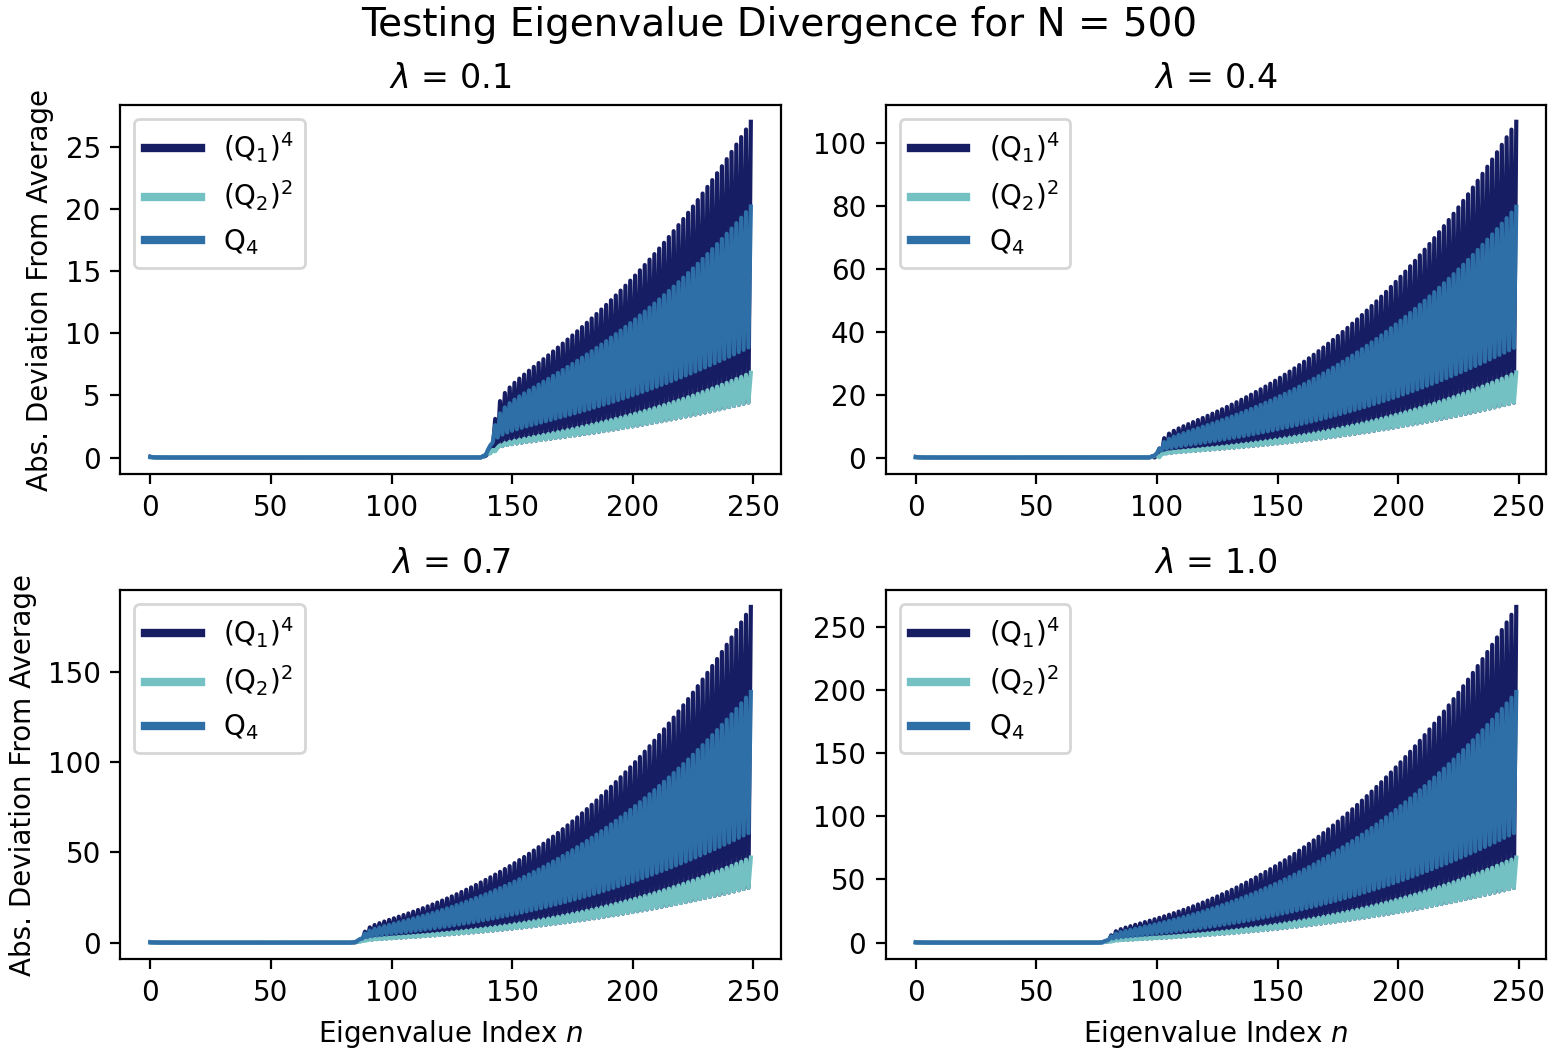
\includegraphics[width=\linewidth]{q1q2q4}
	\caption{Absolute value of the deviation of eigenvalues found with each implementation of $ Q^{4} $ relative to the average value of the three methods together. The deviation diverges for large index $ n $---note the earlier divergence for larger $ \lambda $. See also Table \ref{eigen:table:eigenvalue-convergence}.}
	\label{eigen:fig:q1q2q4-divergence}
\end{figure}


I performed one more test: I found the eigenvalues of a $ 500 \cross 500 $ Hamiltonian using each implementation of $ Q^{4} $, calculated the average value of the three implementations, and then plotted the deviation of each implementation from the average value (see Figure \ref{eigen:fig:q1q2q4-divergence}).

The results surprised me! There are two main takeaways: 
\begin{enumerate}
	\item After a large enough index $ n $ (roughly $ n \approx \frac{N}{4} $), the eigenvalues begin to both oscillate about and diverge exponentially from the average value. In this regime, the eigenvalues transition from linear to roughly exponential growth and grow non-physically large, for example $ E_{500} = \SI{6.57e5}{} $ for $ \lambda = 0.4 $. Table \ref{eigen:table:eigenvalue-convergence} shows the onset index of divergence for various values of the parameter $ \lambda $ and matrix dimension $ N $. 
	
	As a side note, I believe the diverge has something to do with the modification of the Hamiltonian $ H_{0} $ with the perturbation $ Q^{4} $, but---under time pressure---I did not investigate further.
	
	\item For small indices, before the divergent regime, the deviation of each method from the average is essentially zero.\footnote{To be precise, the deviation from the average is of the order $ 10^{-5} $ to $ 10^{-10} $, but this is negligible relative to eigenvalues of order 1 to 100.} In other words, as long the eigenvalues are small enough, the three implementations of $ Q^{4} $ give equivalent results. 
	
\end{enumerate}
With these results in mind, I decided to use $ Q^{4} = \big[(q^{4})_{ij}\big] $ simply because it is fastest. As a bonus, eliminating the need for matrix multiplication when calculating the $ Q^{4} $ should theoretically minimize the accumulation of floating-point arithmetic error relative to the other two options.


\begin{table}[h]
\begin{center}
	\begin{tabular}{c|c c c c}
		$\lambda$ & $ N = 10 $ & $ N = 100 $ & $ N = 500 $& $ N = 1000 $ \\
		\hline
		0.1 & 4 & 38 & 137 & 237 \\
		0.4 & 4 & 25 & 97 & 170 \\
		0.7 & 3 & 21 & 86 & 147 \\
		1.0 & 3 & 19 & 78 & 136
	\end{tabular}
	\caption{Index at which the eigenvalues found with each implementation of $ Q^{4} $ begin to diverge from their average value---see also Figure \ref{eigen:fig:q1q2q4-divergence}. Eigenvalues diverge earlier with both increasing $ \lambda $  at fixed $ N $ and increasing $ N $ at fixed $ \lambda $. Tested with Matlab's \texttt{eig}.}
	\label{eigen:table:eigenvalue-convergence}
\end{center}
\end{table}

\textbf{Two notes:} First, for the remainder of this report, I exclusively calculate $ H $ with $ Q^{4} = \big[(q^{4})_{ij}\big] $. Second, whenever performing analysis on eigenvalues, I considered only those values in the non-divergent regime, shown in in Table \ref{eigen:table:eigenvalue-convergence}.


\subsection{Eigenvalue Methods}


\subsubsection{Overview of What I Implemented By Hand} \label{eigen:sss:methods-by-hand}
Let $ \mat{H} \in \mathbb{R}^{N\cross N} $ be a symmetric matrix. I implemented the following methods by hand:
\begin{itemize}
	\item Two Jacobi methods for finding eigenvalues and eigenvectors without initial tridiagonalization: the classic method in which rotation matrices target the largest absolute value off-diagonal element, and a cyclic version in which the rotation matrices proceed cyclically through $ \mat{H} $.
	
	Applied to $ \mat{H} $, both methods return an eigenvalue matrix $ \mat{D} $ and orthogonal transformation matrix $ \mat{V} $ such that $ \mat{D} = \mat{V}^{T}\mat{A}\mat{V} $ and $ \mat{V} $'s column vectors are $ \mat{A} $'s eigenvalues.
	
	\item QR decomposition using Givens rotations. Returns an orthogonal transformation matrix $ \mat{Q} $ and upper-triangular matrix $ \mat{R} $ such that $ \mat{H} = \mat{Q}\mat{R} $. 
	
	\item An iterative QR eigenvalue method using the above Givens rotation for the QR decomposition. When applied to $ \mat{H} $ returns matrices $ \mat{V} $ and $ \mat{D} $ as described above.

	\item A two-phase algorithm using Householder reflections for tridiagonalization, followed by QR iteration for the final diagonalization. The Householder method returns a tridiagonal matrix $ \mat{T} $ and the corresponding orthogonal transformation matrix $ \mat{P} $ such that $ \mat{T} = \mat{P}^{T}\mat{A}\mat{P} $ and the QR method returns $ \mat{V} $ and $ \mat{D} $ as described above. The complete transformation matrix from $ \mat{H} $ to $ \mat{D} $ is thus $ \mat{Z} = \mat{P}\mat{V} $. 

\end{itemize}
These methods are all generic, so I see no added value in describing them in greater detail here---see the attached source code files for the exact implementation. 


\subsubsection{Stopping Conditions for Iterative Methods}
I exited the iterative QR method when the Hamiltonian matrix's offset value, defined as
\begin{equation*}
	\off(\mat{H}) \equiv \sum_{i\neq j}\abs{\mat{H}_{ij}}^{2},
\end{equation*}
(i.e. the absolute value sum of the off-diagonal elements) fell below a prescribed tolerance $ \epsilon = 10^{-10} $. The choice of $ \epsilon $ is somewhat arbitrary here. I exited the two Jacobi methods on the condition
\begin{equation*}
	\off(\mat{H}_{k}) < \frac{1}{n-1}\left(\frac{\epsilon_{J}}{2n-1}\right)^{2}
\end{equation*}
with $ \epsilon_{J} = 10^{-4} $. This condition guarantees an upper bound of $ \epsilon_{J} $ on the accuracy of all of $ \mat{H} $'s eigenvalues---see page 25 of \cite{chap3}.


\subsection{Eigenvalue Computation Time and Accuracy}
Figure \ref{eigen:fig:times} shows the computation time each method required to diagonalize a single $ N \cross N $ Hamiltonian. Unsurprisingly, Matlab's \texttt{eig} superlatively outperforms all of my ``handmade'' methods. Out of my implementations, the one-phase QR method performed fastest and could reasonably handle matrices up to about $ N \approx 1000 $. The two-phase Householder-QR method completed in a reasonable amount of time up to about $ N \approx 500 $, while the classical Jacobi method failed after $ N \approx 100 $. 

To my pleasant surprise, although the methods' computation times differed by multiple orders of magnitude, the values themselves were nearly identical, as shown in Figure \ref{eigen:fig:error}.

\subsubsection{Brief Case Study: Comparison of Jacobi Methods}
The classical Jacobi method, in which the rotation matrix targets the largest element by absolute value, impressed me by considerably outperforming the cyclic variation, in which the rotation matrix proceed in a prescribed order through the to-be-diagonalized matrix. Figure \ref{eigen:fig:times-jac} compares the two methods---the cyclic method is useful up to about $ N \approx 30 $, while the classical method performs reasonably up to about $ N \approx 100 $.


\begin{figure}[hbt!]
	\centering
	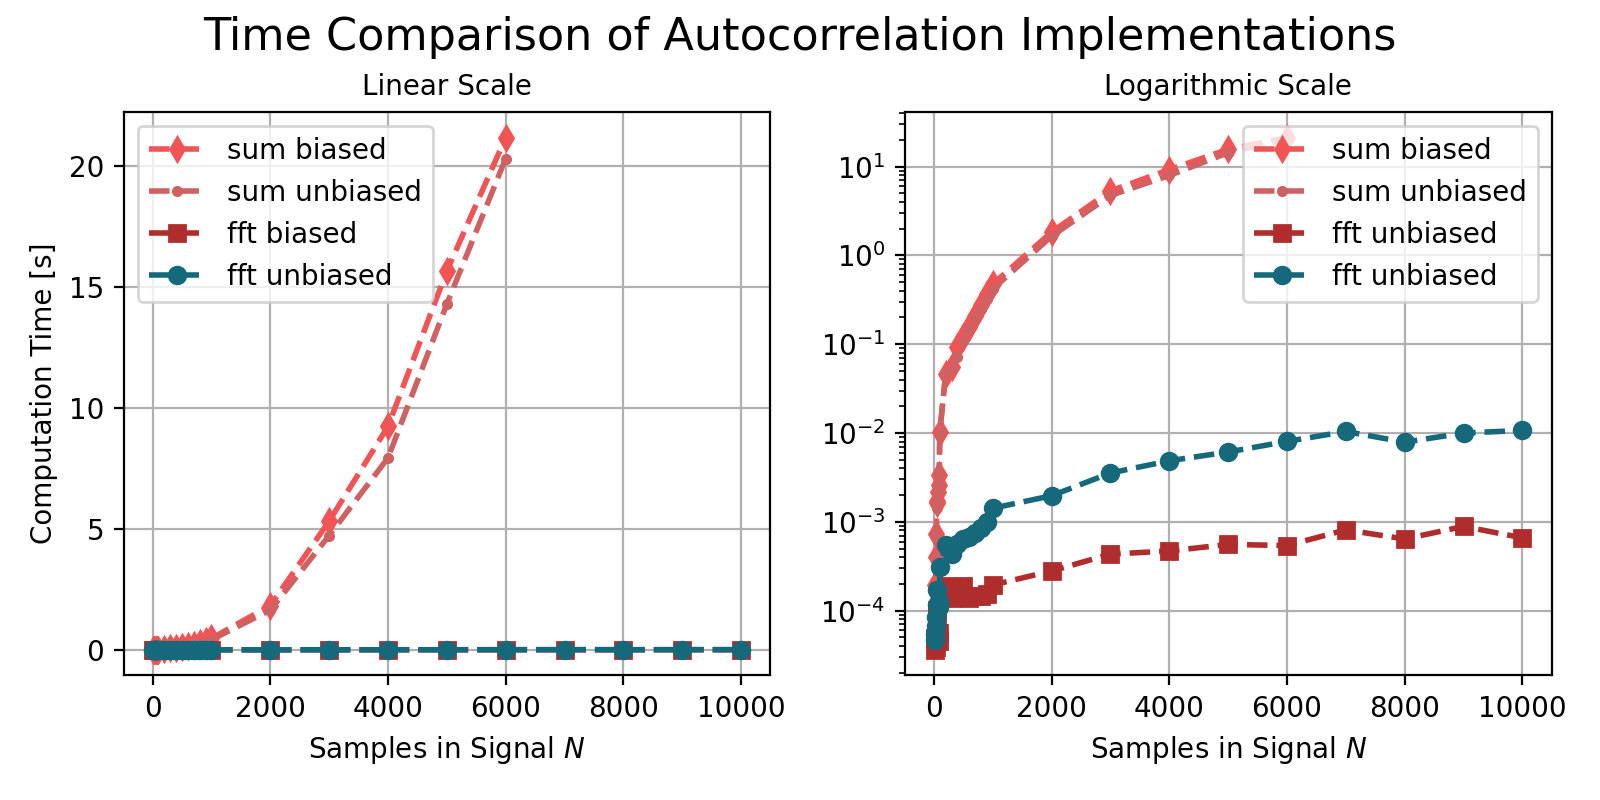
\includegraphics[width=\linewidth]{times}
	\caption{Time required to find the eigenvalues and eigenvectors of an $ N \cross N $ Hamiltonian. Unsurprisingly, Matlab's \texttt{eig} vastly outperforms each of my ``handmade'' implementations.}
	\label{eigen:fig:times}
\end{figure}



\begin{figure}[hbt!]
	\centering
	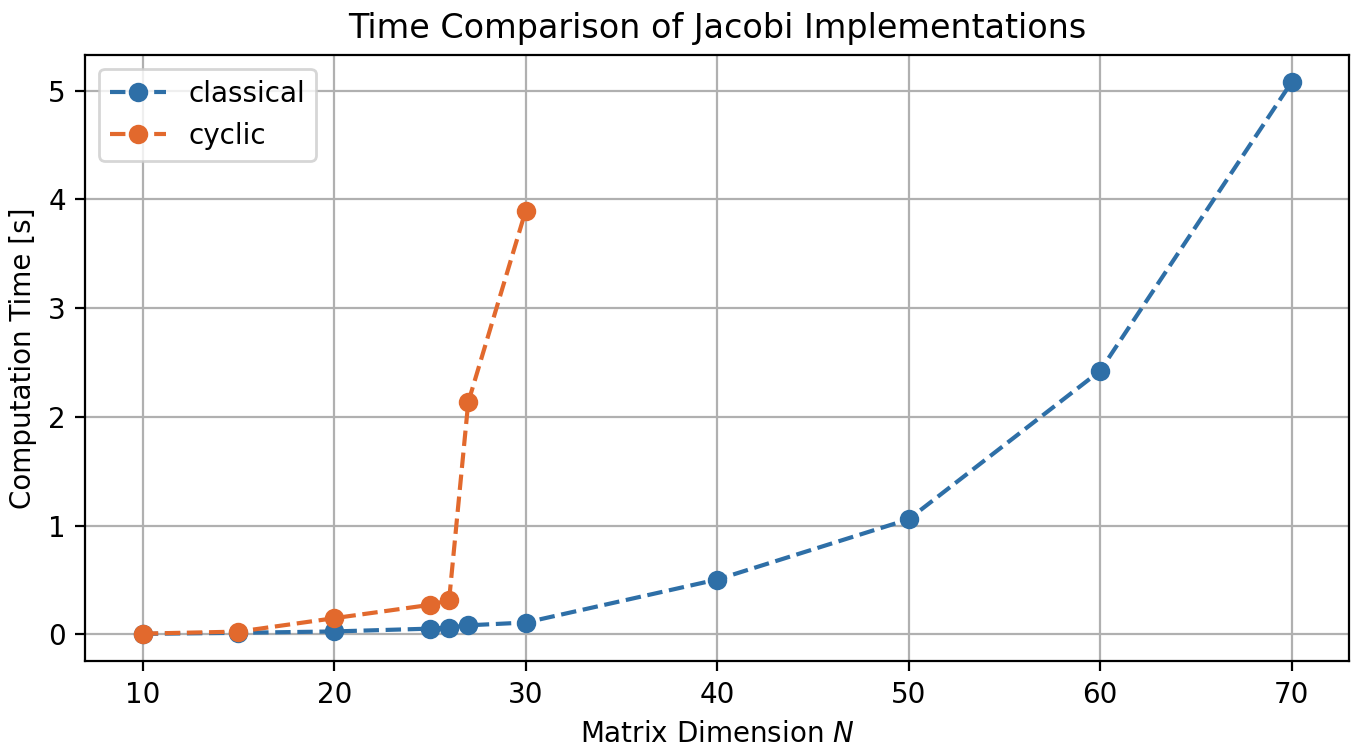
\includegraphics[width=\linewidth]{times-jac}
	\vspace{-5mm}
	\caption{Comparison of the classical and cyclic Jacobi methods (see \hyperref[eigen:sss:methods-by-hand]{Section \ref{eigen:sss:methods-by-hand}}), showing the time required to diagonalize an $ N \cross N $ Hamiltonian.}
	\label{eigen:fig:times-jac}
\end{figure}


\begin{figure}[hbt!]
	\centering
	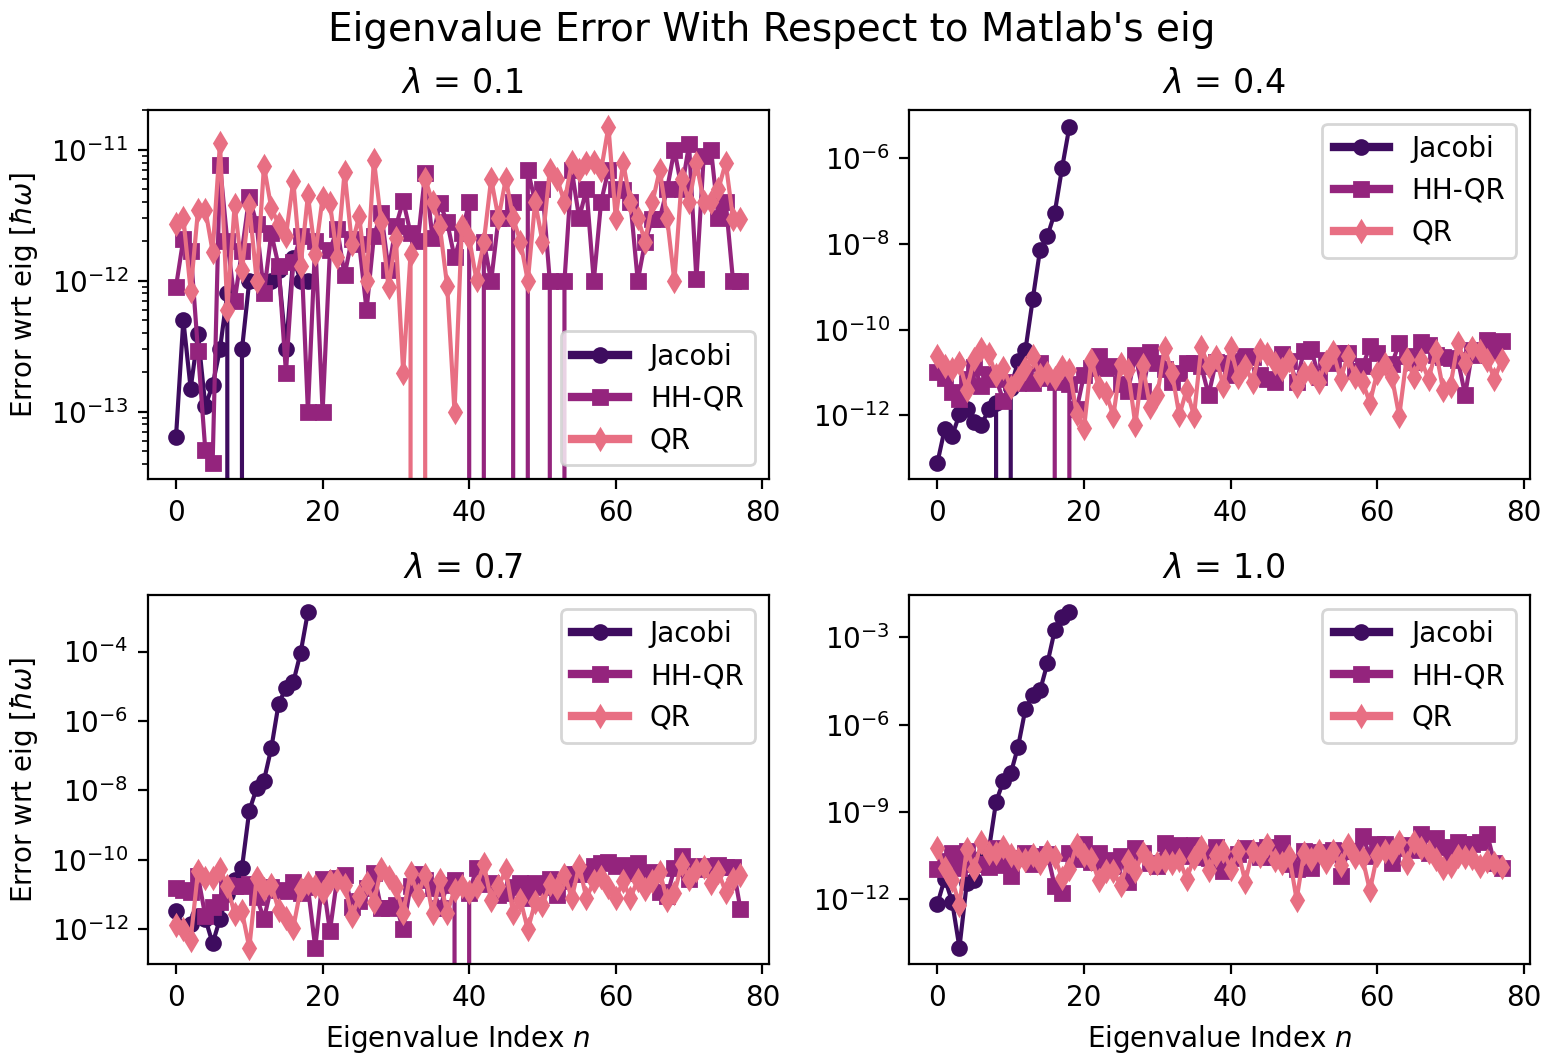
\includegraphics[width=0.97\linewidth]{error} \vspace{-4mm}
	\caption{Absolute deviation of eigenvalues from Matlab's \texttt{eig} for various ``handmade'' implementations. Although the Jacobi method fails for large $ N $, both the Householder and QR methods give the same results as \texttt{eig} to within an impressive $ 10^{-11} $.}
	\label{eigen:fig:error}
\end{figure}
\vspace{-7mm}

\subsection{Eigenvalue, Eigenvector and Eigenfunction Plots}
\textbf{Note:} All eigenvalues (and their associated eigenvectors) displayed in the following figures have been sorted from smallest to largest value. Additionally, all eigenvectors are processed so that the signs of the vector components agree across the \texttt{eig}, QR, two-phase Householder to QR, and Jacobi methods.

\vspace{1mm}
Figure \ref{eigen:fig:eigenvalues} shows $ H $'s first $ \approx 100 $ eigenvalues, while Figure \ref{eigen:fig:eigenvectors-20} shows $ H $'s first $ 20 $ eigenvalues using a colormap on a two dimensional grid. See \hyperref[eigen:s:more-graphs-A]{Appendices \ref{eigen:s:more-graphs-A}} and \ref{eigen:s:more-graphs-B} for many more graphs, including the first 100 eigenvectors for both a single and double-well oscillator; I moved the graphs to the appendix to avoid cluttering the main report.

Figures \ref{eigen:fig:eigenfunc-qho}, \ref{eigen:fig:eigfunc-dw-psi} and \ref{eigen:fig:eigfunc-dw-prob} show the single and double-well oscillator's first few eigenfunctions and probability densities. After diagonalizing the Hamiltonian, I expanded the double-well eigenfunctions in the unperturbed single-well basis from Equation \ref{eigen:eq:qho-basis}, using the components of the $ n $th eigenvector, as abstracted in the following Python code:

\begin{python}
def get_psi_expanded(eigenvector, q):
    """
    Returns an oscillating system's eigenfunction corresponding to the inputted eigenvector by expanding the function in the unperturbed QHO basis 
    """
    psi = np.zeros(len(q))  # preallocate 
    for i in range(0, len(eigenvector)):  # loop through each eigenvector component
        psi += eigenvector[i] * get_psi_qho(i, q)   # linear combination of QHO's i-th basis functions
    return psi
\end{python}


\begin{figure}[hbt!]
	\centering
	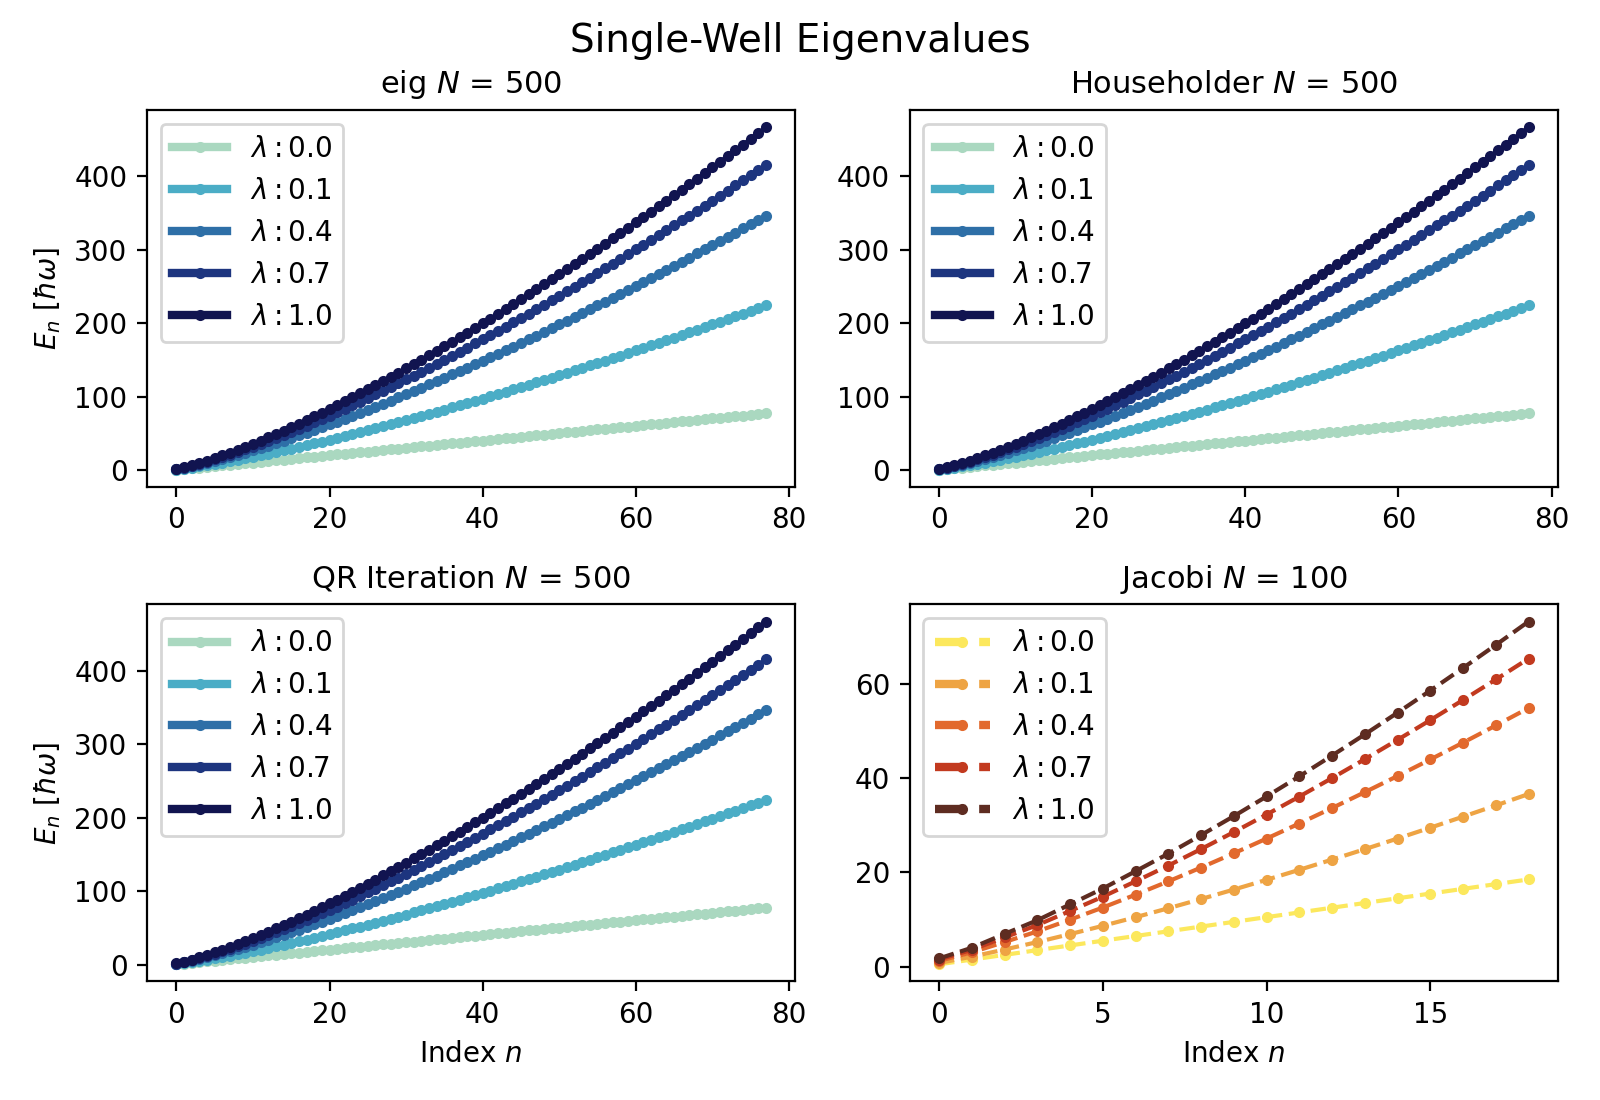
\includegraphics[width=\linewidth]{eigenvalues}
	\caption{Eigenvalues found with various methods. Although $ N = 500 $ (100 for the slower Jacobi method) I only plotted eigenvalues in the non-divergent regime shown in Table \ref{eigen:table:eigenvalue-convergence}. For small $ n $, values found with each method are nearly identical, as shown in Figure \ref{eigen:fig:error}.}
	\label{eigen:fig:eigenvalues}
\end{figure}


\begin{figure}[hbt!]
	\centering
	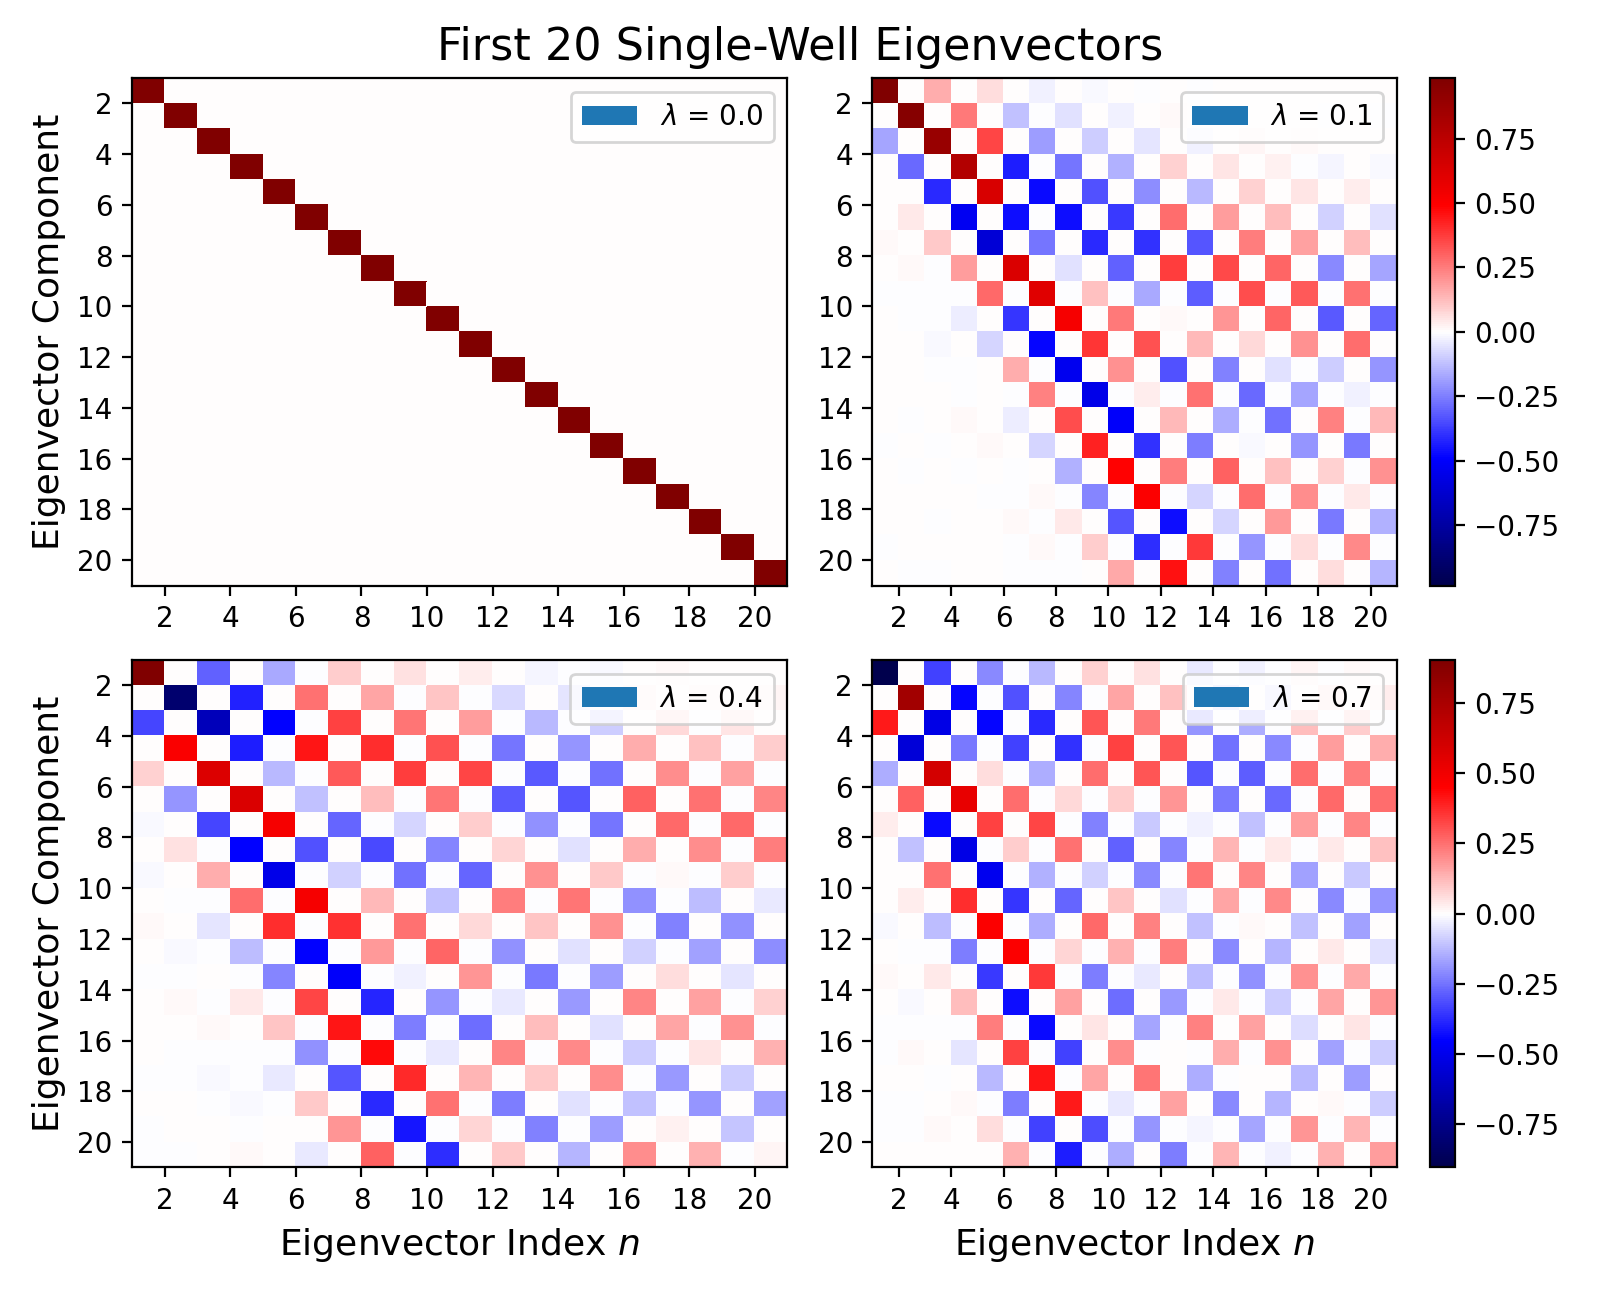
\includegraphics[width=\linewidth]{vectors20}
	\caption{The Hamiltonian's first 20 eigenvectors for various $ \lambda $. The $ n $th eigenvector corresponds to the grid's $ n $th column; red values are positive and blue values are negative. See Figure \ref{eigen:fig:eigenvectors-100} in the Appendix for a plot of $ H $'s first 100 eigenvalues.}
	\label{eigen:fig:eigenvectors-20}
\end{figure}


\subsection{Double-Well Oscillator}
We can model a double-well oscillator the Hamiltonian
\begin{equation*}
	H_{\text{DW}} = \frac{p^{2}}{2} - 2q^{2} + \frac{q^{4}}{10} = \frac{1}{2}(p^{2} + q^{2}) - \frac{5}{2}q^{2} + \frac{q^{4}}{10} = H_{0} - \frac{5}{2}q^{2} + \frac{q^{4}}{10} 
\end{equation*}
I constructed the Hamiltonian in the unperturbed single-well basis using an analogous procedure to the one described in \hyperref[eigen:sss:constructing-Q]{Subsubsection \ref{eigen:sss:constructing-Q}}, using $ \big[(q^{2})_{ij}\big] $ for the $ q^{2} $ term and $ \big[(q^{4})_{ij}\big] $ for the $ q^{4} $ term. The rest of the analysis for the double-well oscillator is analogous to the single-well version described above, and I see no reason to reiterate it here.

Figure \ref{eigen:fig:eigenvalues-double-well} shows the double-well oscillator's first $ \approx 100 $ eigenvalues, while Figure \ref{eigen:fig:eigenvectors-double-well} (in the Appendix) shows the first 20 and 100 eigenvectors, respectively. Note that---unlike for the single-well case---the double-well oscillator's first few eigenvalues are negative.


\begin{figure}[hbt!]
	\centering
	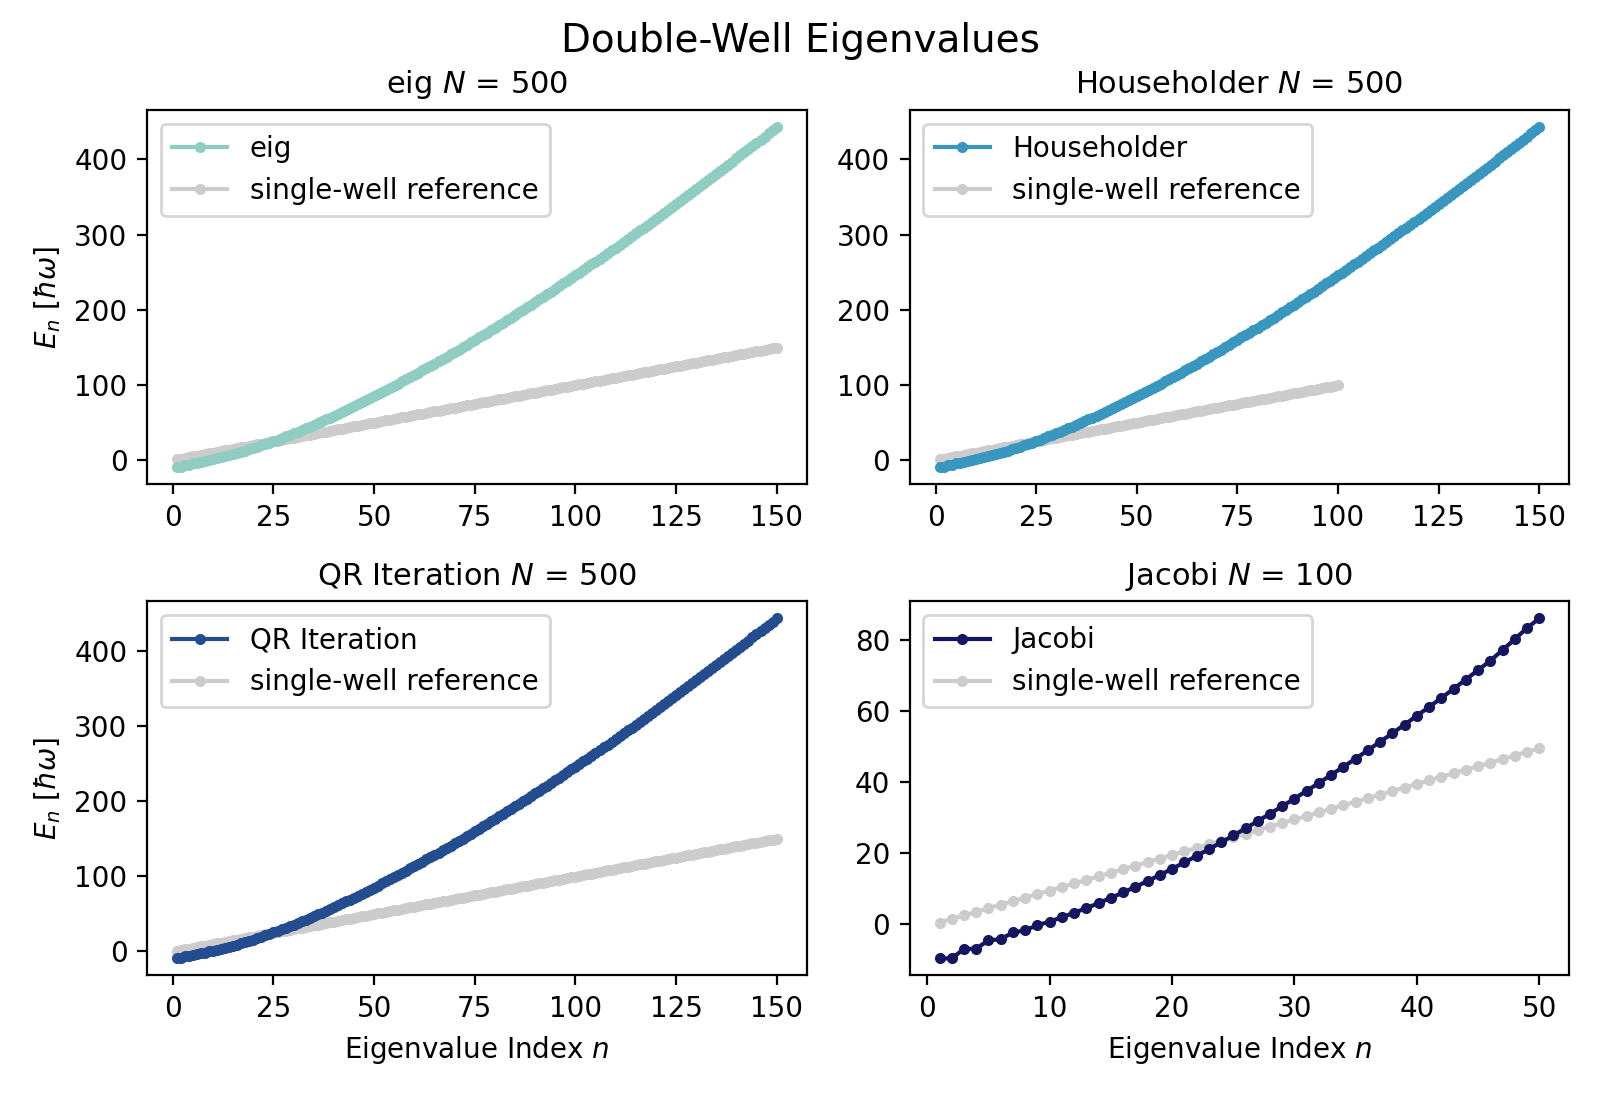
\includegraphics[width=\linewidth]{eigenvalues-double-well}
	\caption{Eigenvalues of the double-well oscillator $ H_{\text{DW}} $ found with various methods. Although $ N = 500 $ (100 for the slower Jacobi method) I only included eigenvalues in the non-divergent regime. The unperturbed single-well eigenvalues are shown for reference.}
	\label{eigen:fig:eigenvalues-double-well}
\end{figure}



\subsection{Some Ideas I Ran Out of Time For}
\begin{itemize}
	\item How would tridiagonalization with Householder reflections compare (speed, accuracy...) to a Hessenberg decomposition, e.g. with Matlab's \texttt{hess}, which returns a tridiagonal matrix for symmetric inputs?
	
	\item Similarly, how does a QR decomposition with Givens rotations compare to Matlab's  built-in \texttt{qr}?
	
	\item Compare the speed of a traditional QR iterative eigenvalue method to an implementation using Wilkinson shifts (see e.g. \cite{qr}).
	
\end{itemize}







\appendix

\section{More Eigenvector Plots} \label{eigen:s:more-graphs-A}
I'm including these here to avoid cluttering the main report with erratically placed figures.


\begin{figure}[htb!]
	\centering
	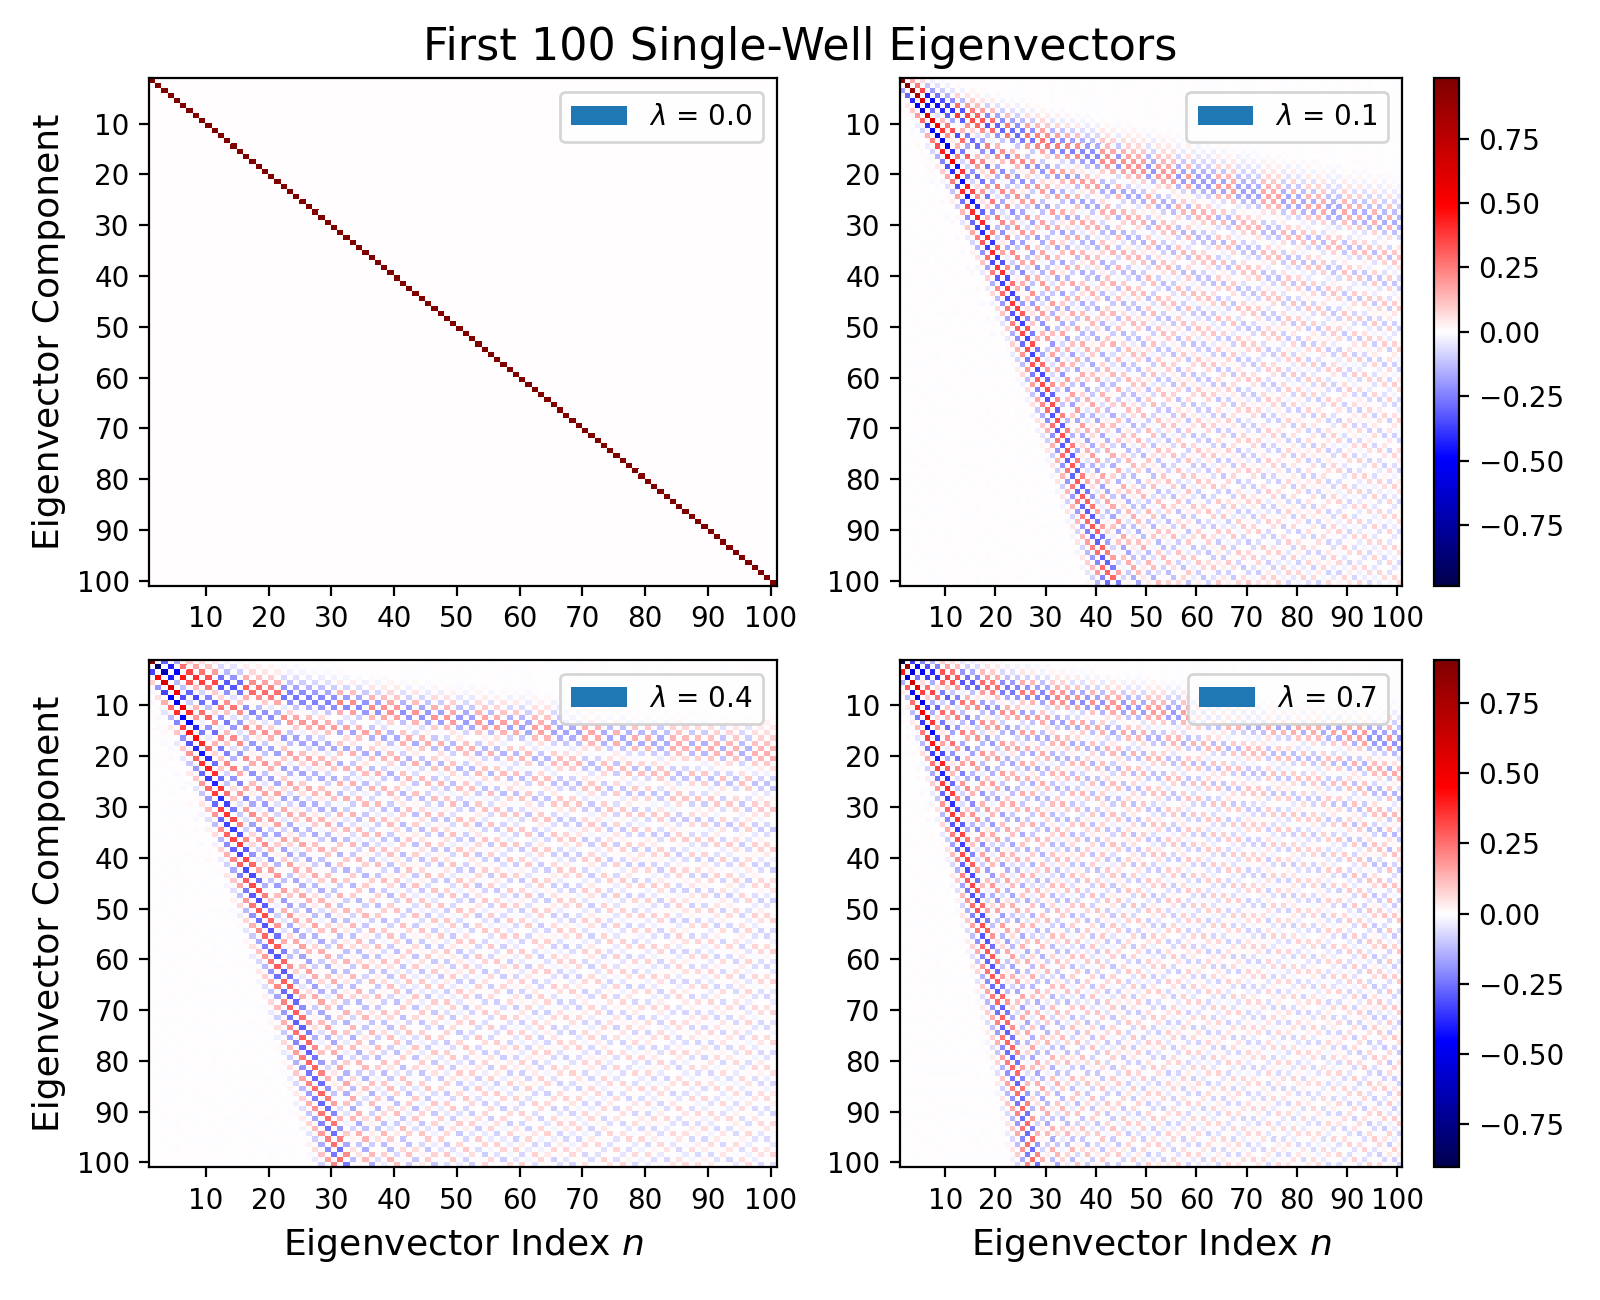
\includegraphics[width=\linewidth]{vectors100}
	\caption{The perturbed Hamiltonian's first 100 eigenvectors for various $ \lambda $. The $ n $th eigenvector corresponds to the grid's $ n $th column; red values are positive and blue values are negative. Note the principle (more intensely colored) components' increasing divergence from the unperturbed linear trend as $ \lambda $ increases.}
	\label{eigen:fig:eigenvectors-100}
\end{figure}

\begin{figure}[htb!]
	\centering
	{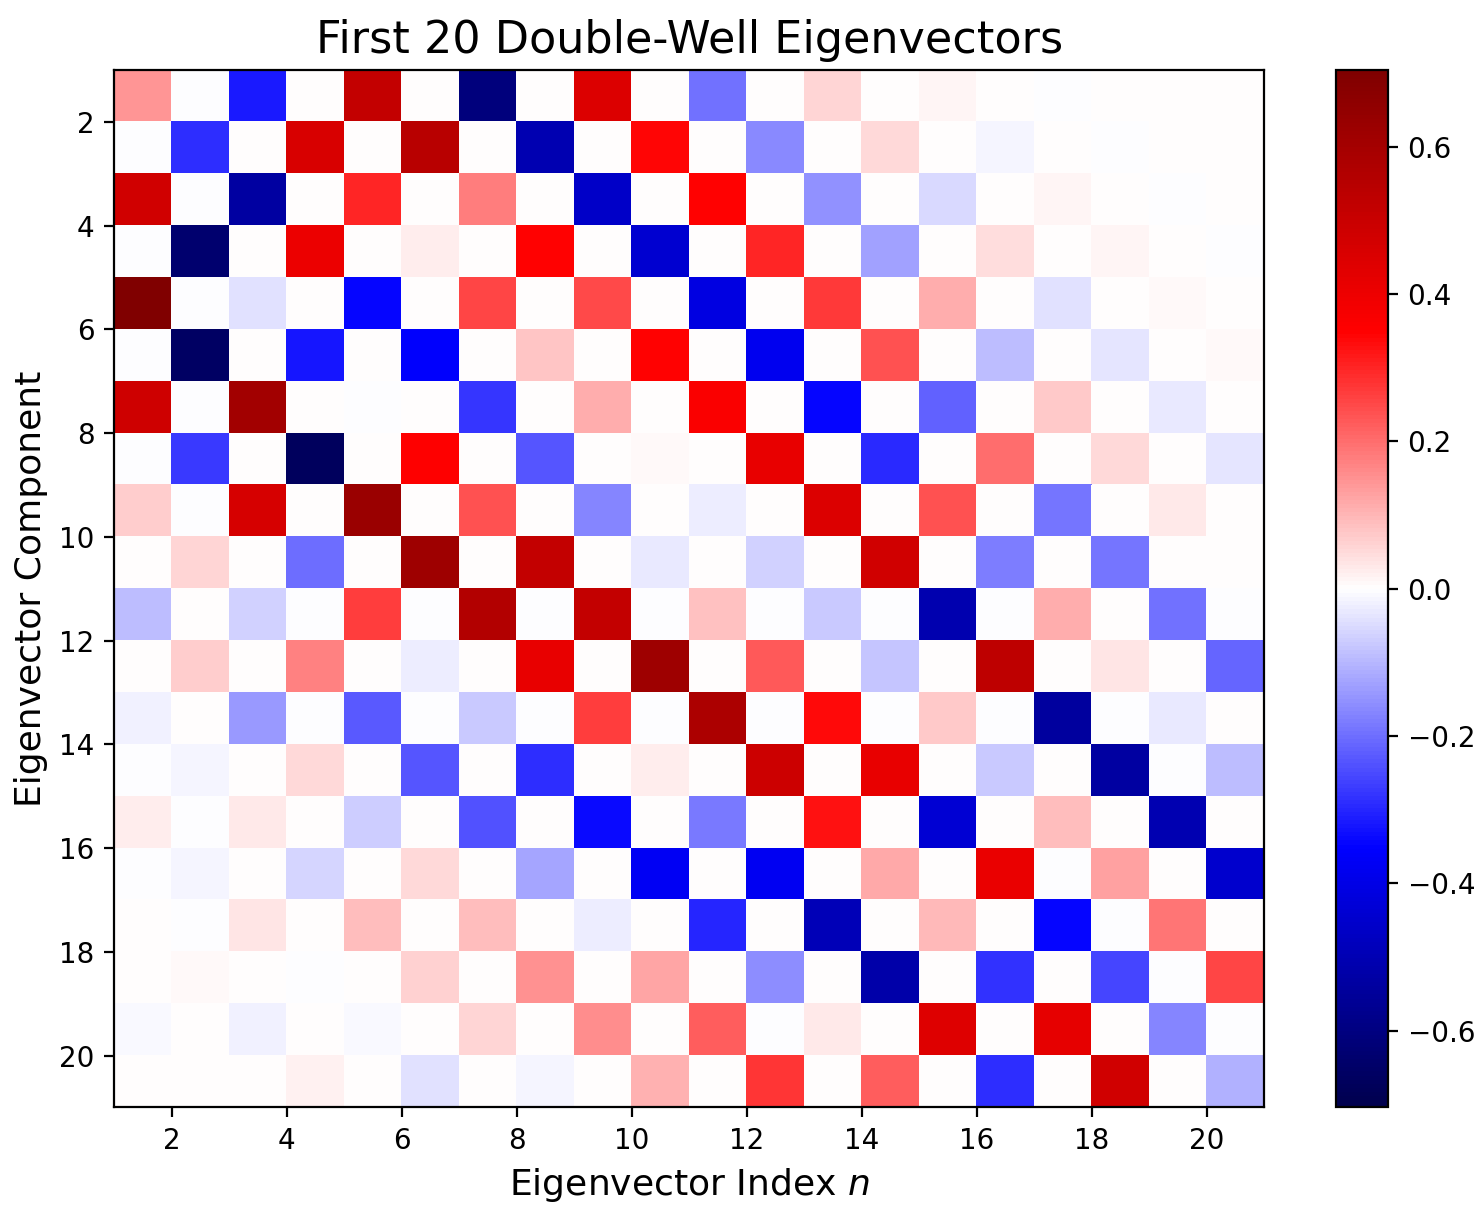
\includegraphics[width=0.9\linewidth]{vectors-double-well20}}\vfill 
	
	{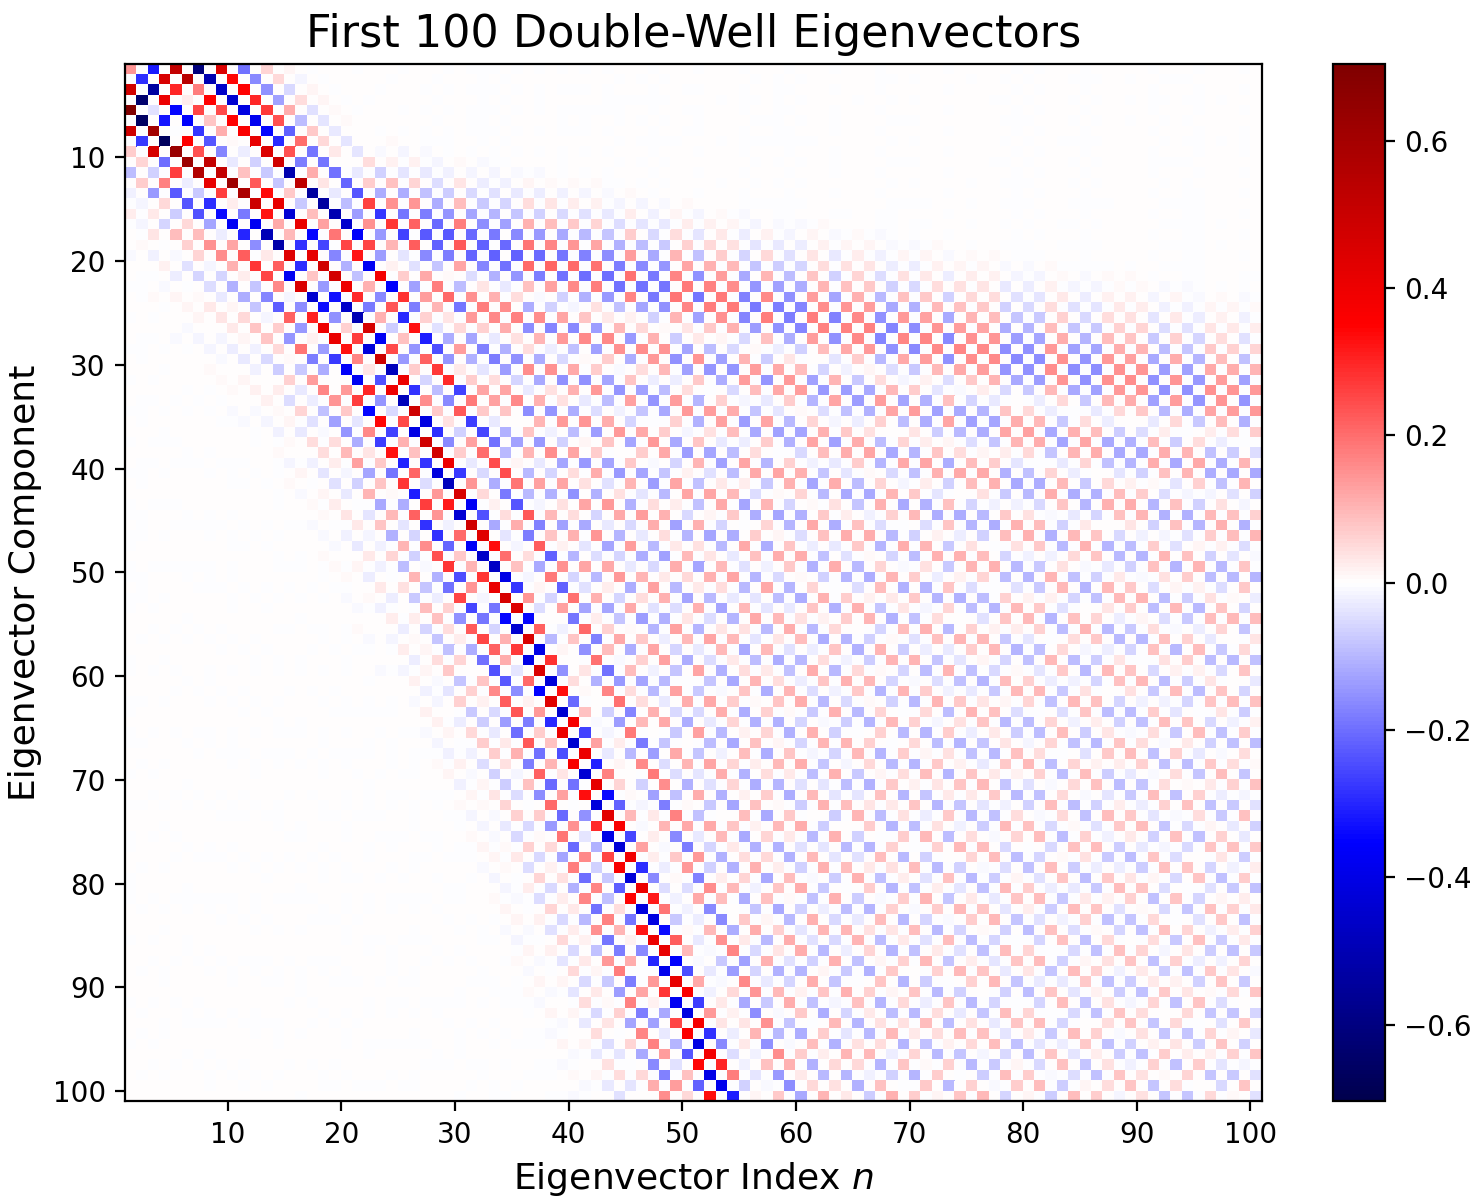
\includegraphics[width=0.9\linewidth]{vectors-double-well100}}\vfill
	
	\caption{The double-well Hamiltonian's first 20 and 100 eigenvectors. The $ n $th eigenvector corresponds to the grid's $ n $th column. The two diagonal bands of principle (more intensely-colored) components appear slightly wider than in the single-well case in Figure \ref{eigen:fig:eigenvectors-100}, indicating more $ \ket{n^{0}} $ basis functions contribute appreciably to the double-well oscillator.}
	\label{eigen:fig:eigenvectors-double-well}
\end{figure}

\section{Eigenfunction Plots} \label{eigen:s:more-graphs-B}


\begin{figure}[htb!]
	\centering
	{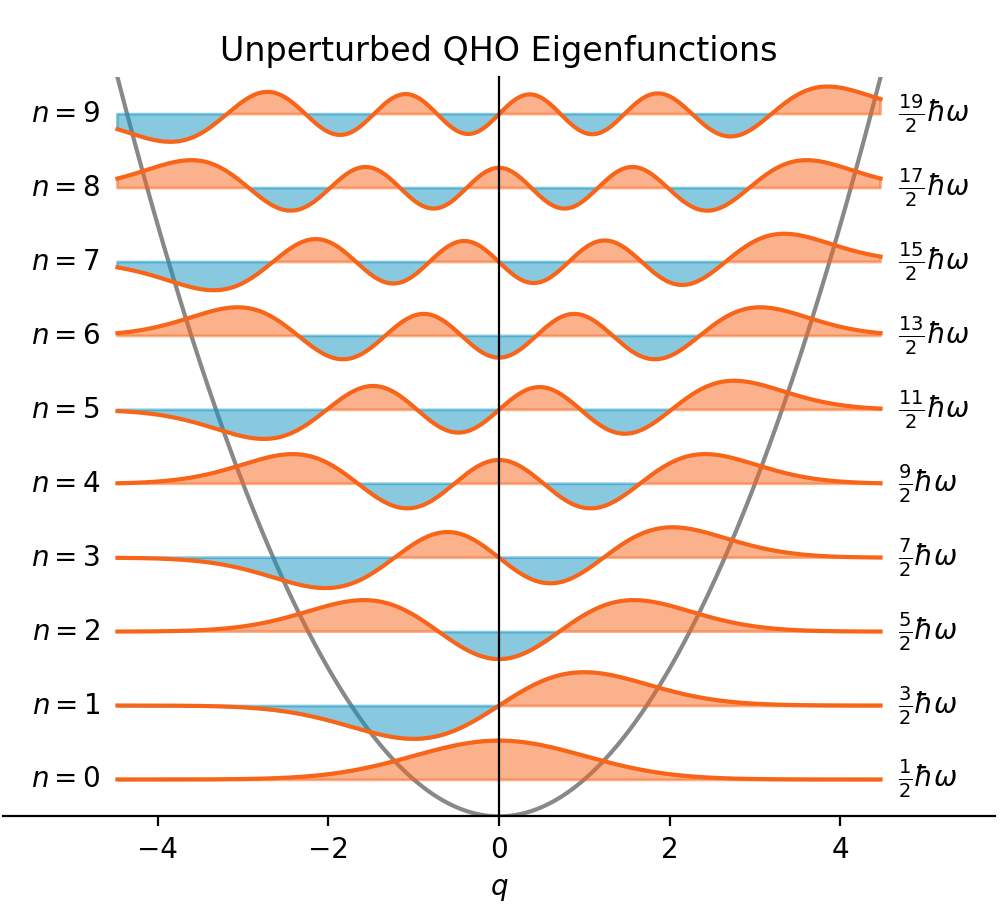
\includegraphics[width=.48 \textwidth]{eigfunc-qho-psi}}\hfill  % use vfill for vertically spaced images
	{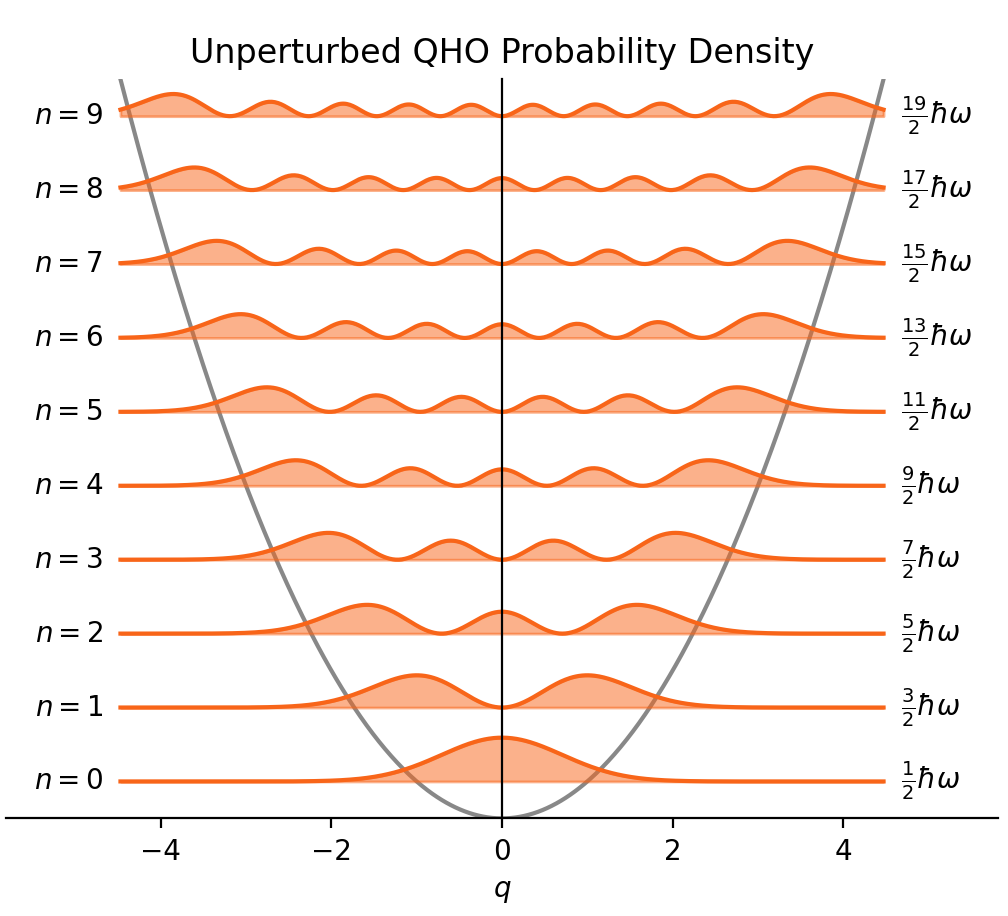
\includegraphics[width=.48 \textwidth]{eigfunc-qho-prob}}\hfill
	\caption{The unperturbed harmonic oscillator's first few eigenfunctions $ \psi_{n} $ and probability densities $ \abs{\psi_{n}}^{2} $, which nicely show the QHO's linear increase of $ E_{n} $ with $ n $.}
	\label{eigen:fig:eigenfunc-qho}
\end{figure}




\begin{figure}[htb!]
	\centering
	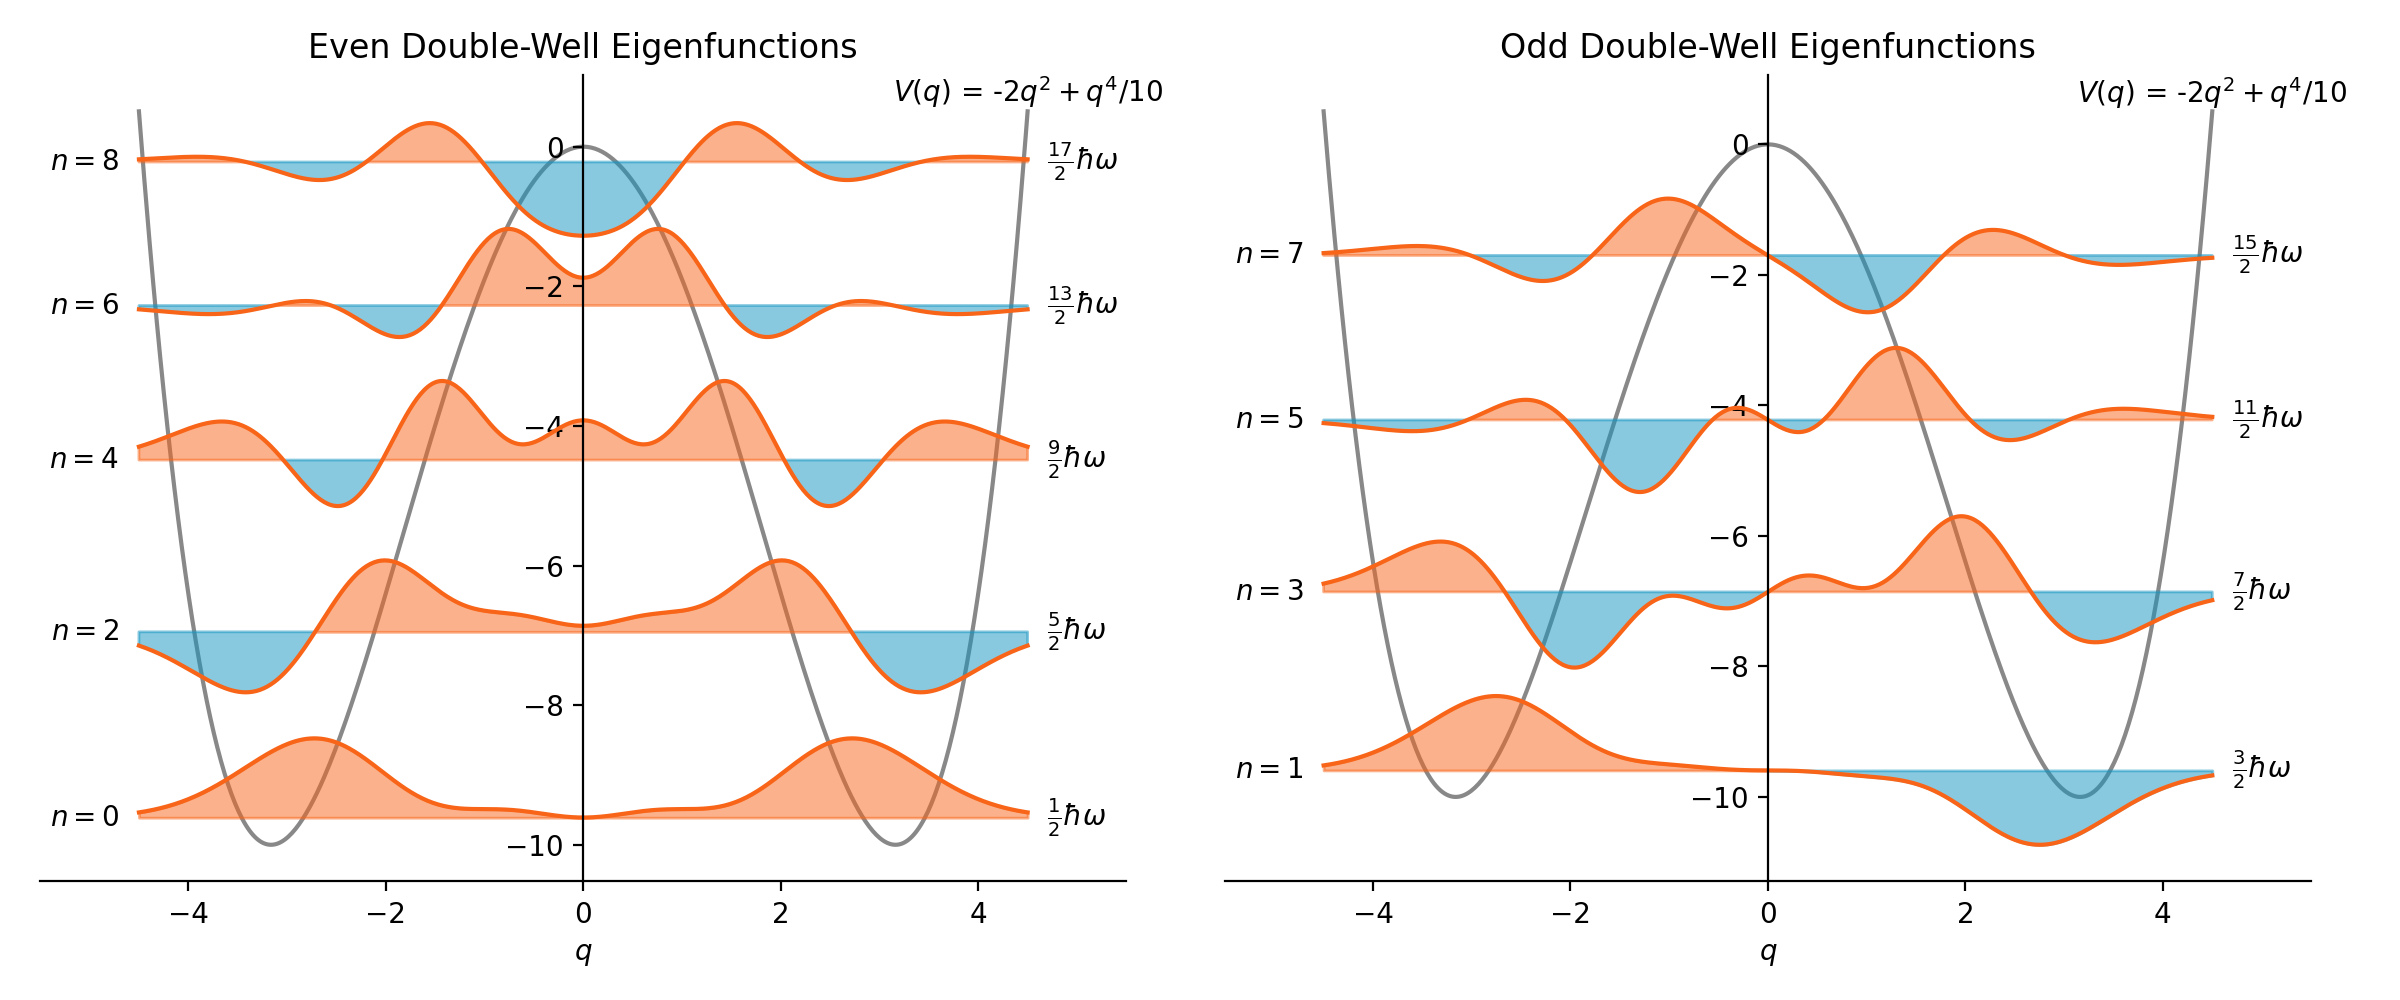
\includegraphics[width=\linewidth]{eigfunc-dw-subplots-psi}
	\caption{The double-well Hamiltonian's first few eigenfunctions---note that the first few eigenvalues are negative. The even and odd functions are separated to avoid overlap.}
	\label{eigen:fig:eigfunc-dw-psi}
\end{figure}

\begin{figure}[htb!]
	\centering
	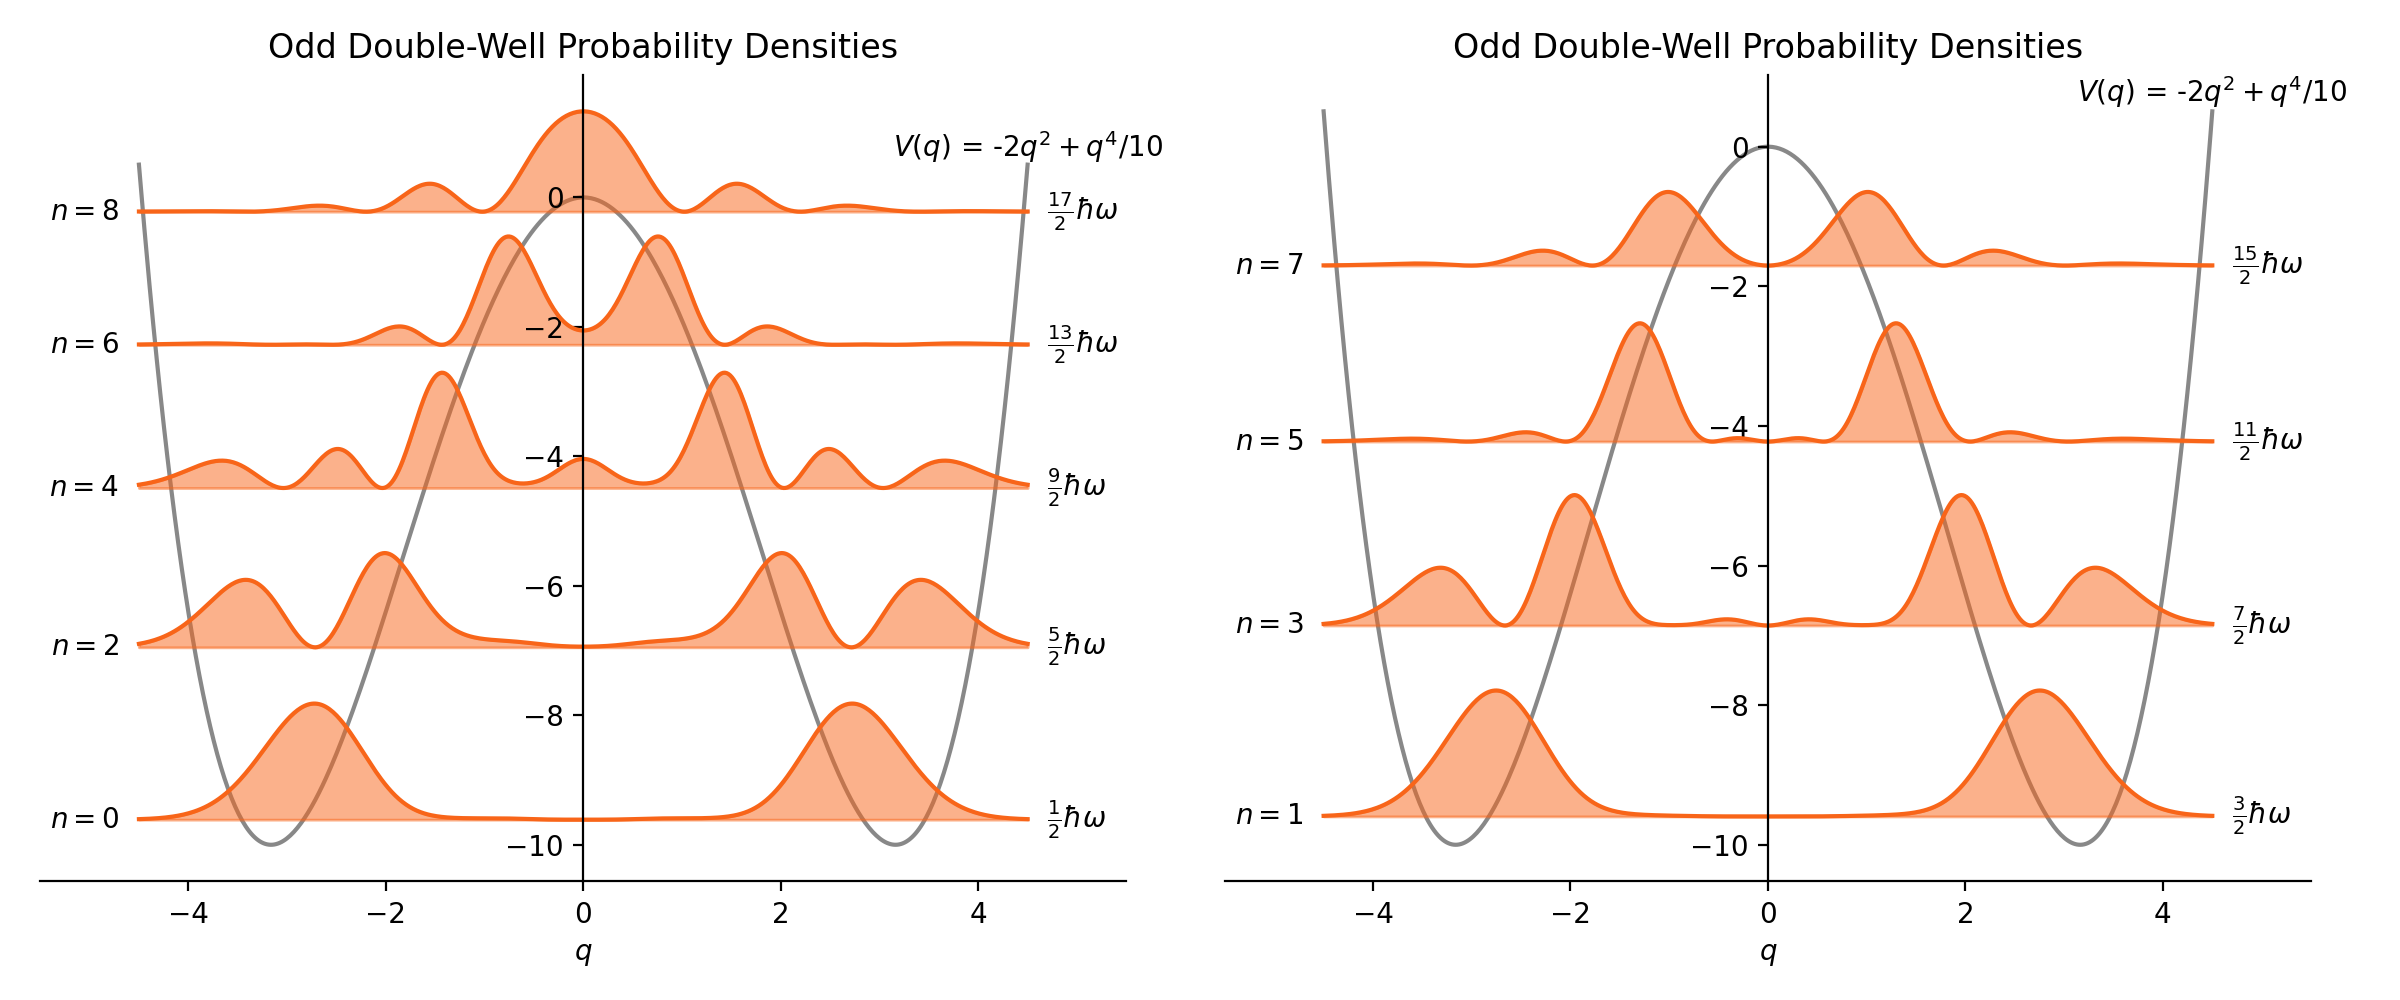
\includegraphics[width=\linewidth]{eigfunc-dw-subplots-prob}
	\caption{The double-well Hamiltonian's first few probability densities, i.e. $ \abs{\psi_{n}}^{2} $. The even and odd functions are separated to avoid overlap.}
	\label{eigen:fig:eigfunc-dw-prob}
\end{figure}

\iffalse

\section{The Symmetric Eigenvalue Problem}
This section is fairly basic, but it still helped me to review the fundamentals, so I'm including it here.
\begin{itemize}
	\item Given $ \mat{A} \in \mathbb{R}^{n \cross n} $, the \textit{eigenvalue problem} refers to finding all pairs $ (\lambda, \vec{v}) $ of scalars $ \lambda \in \mathbb{R} $ and vectors $ \vec{v} \in \mathbb{R}^{n} $ that together satisfy the equation
	\begin{equation*}
		\mat{A} \vec{v} = \lambda \vec{v}
	\end{equation*}
	The scalar values $ \lambda_{i} $ satisfying the equation are called $ \mat{A} $'s \textit{eigenvalues}. The corresponding vectors $ \vec{v}_{i} $ are called $ \mat{A} $'s \textit{eigenvectors}. 
	
	Note that eigenvectors are defined only up to a constant factor. By convention, we remove ambiguity by requiring the eigenvectors are normalized, i.e. $ \norm{\vec{v}} = 1 $. The set of $ \mat{A} $'s eigenvalues is called $ \mat{A} $'s \textit{spectrum}, and is usually denoted by $ \sigma(A) $.
	
	\item In practice, we solve the eigenvalue problem by finding a transformation matrix $ \mat{Z} \in \mathbb{R}^{n \cross n} $ solving the equation
	\begin{equation*}
		\mat{A} \mat{Z} = \mat{Z} \mat{D} \eqtext{or} \mat{Z}^{-1}\mat{A}\mat{Z} = \mat{D}
	\end{equation*}
	where $ \mat{D} = \diag(\lambda_{1}, \lambda_{2}, \ldots, \lambda_{n}) $ is a diagonal matrix whose diagonal entries are $ \mat{A} $'s eigenvalues. If we can find such a $ \mat{Z} $, then $ \mat{Z} $'s columns are $ \mat{A} $'s eigenvectors, and the vector in $ \mat{Z} $'s $ i $th column corresponds to the eigenvalue in $ \mat{D} $'s $ i $th column. 
	
	$ \mat{Z} $ is a transformation matrix that transforms $ \mat{A} $ into the diagonal matrix $ \mat{D} $. 
	
	\item If $ \mat{A} $'s eigenvectors $ \vec{v}_{i} $ are orthogonal, then $ \mat{Z} $ is an orthogonal matrix and the eigenvalue equation reads
	\begin{equation*}
		\mat{Z}^{T}\mat{A}\mat{Z} = \mat{D}
	\end{equation*}
	\textit{The eigenvalue problem becomes transforming $ \mat{A} $ into a diagonal matrix $ \mat{D} $.}
	In practice, we transform $ \mat{A} $ into diagonal form in steps, using a sequence of orthogonal transformations $ \mat{P}_{k} $. At the first iteration, we have
	\begin{equation*}
		\mat{A} \to \mat{P}_{1}^{T}\mat{A}\mat{P}_{1}
	\end{equation*}
	after the second iteration, we have
	\begin{equation*}
		\mat{A} \to \mat{P}_{2}^{T}\mat{P}_{1}^{T}\mat{A}\mat{P}_{1}\mat{P}_{2}
	\end{equation*}
	and so on. The hope is that after enough properly chosen transformations $ \mat{P}_{k} $, we will reach the perfectly diagonal form $ \mat{Z}^{T}\mat{A}\mat{Z} = \mat{D} $. In this case
	\begin{equation*}
		\mat{Z} = \mat{P}_{1}\mat{P}_{2}\mat{P}_{3}\cdots
	\end{equation*}
	The eigenvalue problem thus boils down to properly choosing the transformation matrices $ \mat{P}_{k} $ so that $ \mat{A} $ will become diagonal.
	
\end{itemize}
\fi

\begin{thebibliography}{}
\setlength{\itemsep}{.2\itemsep}\setlength{\parsep}{.5\parsep}

\bibitem{chap3} Carlsen, Eric. \textit{Chapter 3 of Calculus$^{++}$: The Symmetric Eigenvalue Problem}. Georgia Institute of Technology. (2006). \url{https://www.math.wustl.edu/~wick/teaching/Math2605Notes/chap3.pdf}.

\bibitem{qr} Townsend, Alex. \textit{The QR Algorithm}. (2019). \url{http://pi.math.cornell.edu/~web6140/TopTenAlgorithms/QRalgorithm.html}

\bibitem{C-recipes} William H. Press, et al. \textit{Numerical Recipes in C: the Art of Scientific Computing}. Cambridge; New York: Cambridge University Press, 1992.

\bibitem{wilkinson} Wilkinson, J. H.. \textit{The Algebraic Eigenvalue Problem}. (1965).


\end{thebibliography}


\end{document}

% Wavefunctions graph: https://scipython.com/blog/the-harmonic-oscillator-wavefunctions/

